\documentclass{article}
\usepackage[utf8]{inputenc}
\usepackage{wrapfig}
\usepackage{graphicx}
\usepackage{setspace}
\usepackage{lipsum}
\usepackage[skip=0.333\baselineskip]{caption}
\usepackage{subcaption}
\usepackage[colorlinks=true, linkcolor=blue, citecolor=blue, urlcolor=blue]{hyperref}
\usepackage[style=numeric,backend=bibtex,giveninits=true,terseinits=true,doi=false,url=false,isbn=false]{biblatex}
\usepackage{geometry}
\geometry{top=1in, bottom=1in, left=0.75in, right=0.75in}


\title{\textbf{\Large Improving SNR and Resolution in LiDAR by matrix-based analysis}}

\author{
    \textbf{Benzy Laufer} \\  Supervisor - Prof. Ori Katz \\
    Institute of Applied Physics, The Hebrew University of Jerusalem. 
}


\bibliography{ref}

\begin{document}

% \setstretch{0.9}

\date{}

\maketitle

\section{Introduction}
\large Light Detection and Ranging (LiDAR) technology is a popular solution for a wide variety of applications, from atmospheric sensing, through 3D shape measurements, to autonomous vehicles. LiDAR has the unique ability to map the space around it in three dimensions (3D) and high sensitivity, making it possible to identify road hazards with high spatial and temporal resolution even in harsh conditions. This is achieved by scanning a pulsed or temporally modulated laser beam over the scene and measuring the arrival time of the reflected beam.

However, LiDAR scanning faces two fundamental challenges:
\begin{enumerate}
    \item The long distance to the target and the limited aperture size of the light-collecting optics result in very weak signals, particularly in harsh conditions such as foggy or dusty scenes.
    \item When illuminating a point in the scan, the scanning beam illuminates an area whose size is optimally defined by the diffraction-limit, limited by the transmitter aperture. Additionally, optical distortions and aberrations in the path between the transmitter and the target can further enlarge this area, ultimately limiting the spatial resolution of any LiDAR system.
\end{enumerate}

\section{Methodology}
In my PhD, I will investigate the adaptation and development of advanced matricial techniques to LiDAR imaging. Such matrix-based approaches have been recently proved by our group and others to significantly improve resolution, signal to noise (SNR), and image quality in several fields of imaging, from optical microscopy \cite{Badon2020}, through ultrasound \cite{PhysRevX.10.021048}, to seismology \cite{2018JB016361}. The approaches that I will investigate include Image Scanning Microscopy (ISM) \cite{muller} and aberration estimation and correction \cite{Badon2020}. Matrix-based approaches have so far not impacted the important field of LiDAR imaging, mainly because it requires multi-pixel detection. The improvement in multipixel sensitive detector technology now allows implementing such detection, which opens the path to this work.

%both theoretically and numerically, and implement it in an experimental proof-of-principle experiment in our lab. ISM, also known as "pixel reassignment," was developed to improve the SNR and resolution in a confocal microscope. 
%At this stage, we have conducted simulations specifically for the ISM method, but we may explore other methods within the Matrix approach as our research progresses. The Matrix approach has been applied in various fields, such as optical microscopy, ultrasonic imaging, and seismic imaging.

Currently, there are two common detection approaches in LiDAR:
\begin{enumerate}
    \item[a.] Confocal detection: A small detector is used to optimally detect only the light returning from a small area around the illumination point.
\item[b.] Large ("bucket") detection: where all incoming light is detected.
\end{enumerate}

While confocal detection offers improved resolution and out-of-focus background rejection, which may be significant in foggy conditions, it may collect substantially less reflected light, resulting in a lower signal-to-noise ratio (SNR).

My research will combine theoretical and numerical investigation in addition to experimental proof-of-principle experiments. As the first stage of my work, I will study the possibility of combining the advantages of both methods by adapting ISM originally developed for optical microscopy. With proper adaptation, it is expected to improve both resolution and SNR in scanning LiDAR with a very straighforward computation step.

In short, in ISM, all the light reflected from the target is detected using an array of detectors while the beam is scanned over the scene. While the signal from the central detector provides the confocal (low SNR) image, the signals from the neighboring detectors are 'reassigned' using a simple computation to improve the SNR while improving the imaging resolution.

\section{Preliminary Results}
In my short work so far, I have performed a preliminary numerical investigation of ISM using a Python-based numerical simulation that I have developed. 
The preliminary simulation results presented in Fig.1  demonstrate that ISM imaging outperforms confocal imaging, which by itself outperforms bucket-based LiDAR imaging. These encouraging findings support the potential benefits of incorporating this basic matricial approach into scanning LiDAR systems.

Following the experimental proof-of-principle demonstration of ISM in free space, we will further examine additional possibilities for improving LiDAR in cases of scattering and atmospheric aberrations, as is present in many actual scenarios. Tackling this important challenge, which has a huge societal impact, will be done by leveraging more advanced matricial approaches, such as those very recently presented to overcome aberration and scattering in optical coherence tomography (OCT) \cite{Badon2020}, ultrasound  imaging \cite{PhysRevX.10.021048} and seismology\cite{2018JB016361}, and which represent the state-of-the-art in wave-based imaging.% ring medium and coherence microscopy, particularly Optical Coherence Tomography (OCT), to obtain surface topography with higher resolution than currently available techniques.

%In our preliminary results, we have conducted simulations that generated the images shown in Figure \ref{fig:roc}, illustrating the differences between original, wide field, confocal, and ISM imaging. These simulation results highlight the potential advantages of incorporating the Matrix approach, especially ISM, into scanning LiDAR systems.

\begin{figure}[hbt!]
\centering
\begin{minipage}{.225\linewidth}
\centering
\captionsetup{type=figure}
Target \

\includegraphics[width=\linewidth]{001 Object.png}
\label{subfig:original}
\end{minipage}\hfill
\begin{minipage}{.225\linewidth}
\centering
\captionsetup{type=figure}
Conventional LiDAR \
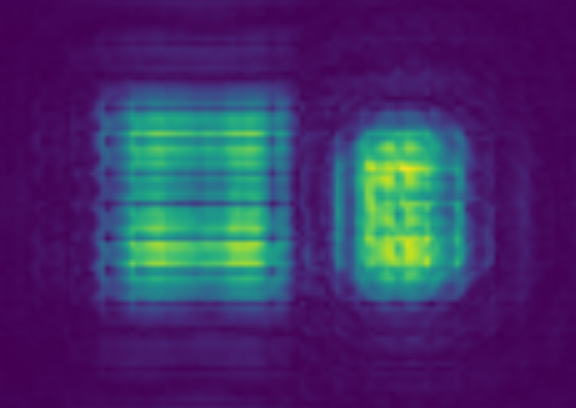
\includegraphics[width=\linewidth]{002 wide field imaging.png}
\label{subfig:widefield}
\end{minipage}\hfill
\begin{minipage}{.225\linewidth}
\centering
\captionsetup{type=figure}
Confocal LiDAR \
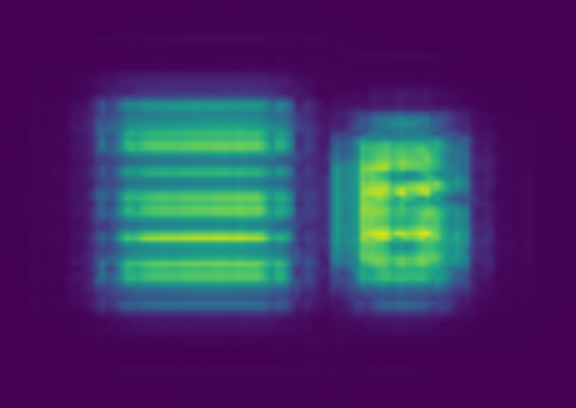
\includegraphics[width=\linewidth]{003 confocal imaging.png}
\label{subfig:confocal}
\end{minipage}\hfill
\begin{minipage}{.225\linewidth}
\centering
\captionsetup{type=figure}
Our approach \
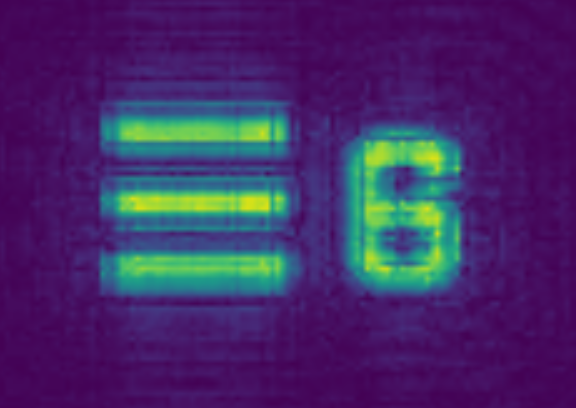
\includegraphics[width=\linewidth]{004 ism imaging.png}
\label{subfig:ism}
\end{minipage}
\caption{Comparison of different imaging techniques.}
\label{fig:roc}
\end{figure}

%\blfootnote{[1] Muller et al., PRL 104 (19 2010), p. 198101.}

\printbibliography

\end{document}